\documentclass[12pt]{article}
\usepackage{graphicx}

\title{Labwork 3 Report: Hello, CUDA!}
\author{Le Hoai Nam \\ Student ID: 2540079}
\date{\today}

\begin{document}

\maketitle

\section{Introduction}
In this labwork, I implemented an RGB-to-grayscale image converter using Python, comparing CPU execution with Numba CUDA GPU acceleration.

\section{Implementation}
The image is loaded using \texttt{matplotlib.pyplot.imread} and reshaped into a 1D array of RGB values \texttt{(pixelCount, 3)}.

\begin{itemize}
    \item \textbf{CPU Version:} A standard \texttt{for} loop calculates the luminance $0.299R + 0.587G + 0.114B$ for each pixel[cite: 5].
    \item \textbf{GPU Version:} A CUDA kernel processes each pixel in parallel across multiple threads[cite: 5].
\end{itemize}

Pseudocode of the CUDA kernel[cite: 5]:
\begin{verbatim}
i = threadIdx.x + blockIdx.x * blockDim.x
if i < total_pixels:
    gray = 0.299 * src[i, 0] + 0.587 * src[i, 1] + 0.114 * src[i, 2]
    dst[i, 0] = dst[i, 1] = dst[i, 2] = gray
\end{verbatim}

\section{Results}
The test was conducted on an NVIDIA GeForce GTX 1050 GPU.

\begin{figure}[h]
    \centering
    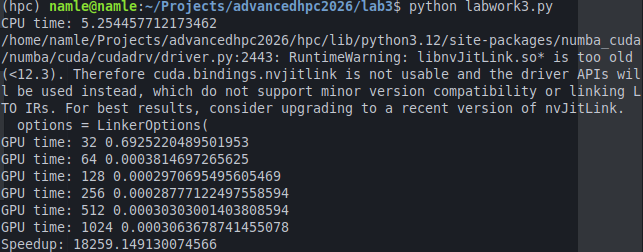
\includegraphics[width=0.75\textwidth]{result.png}
    \caption{Result}
\end{figure}

\begin{itemize}
    \item \textbf{CPU Time:} 5.2545 seconds[cite: 5]
    \item \textbf{GPU Time (Block Size 256):} 0.000288 seconds[cite: 5]
    \item \textbf{Speedup:} ~18259x[cite: 5]
\end{itemize}

\begin{figure}[h]
    \centering
    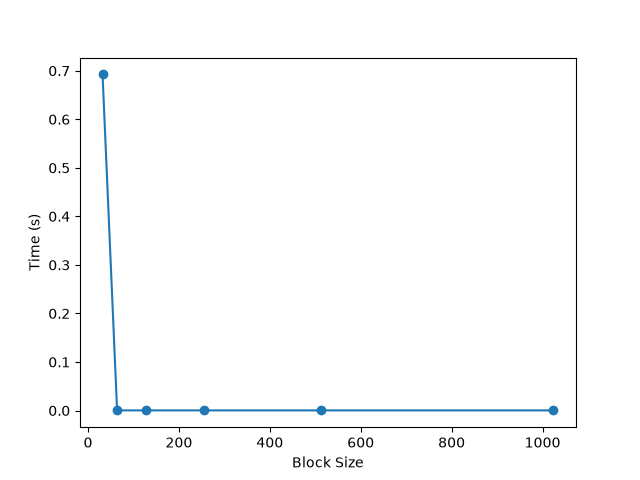
\includegraphics[width=0.75\textwidth]{block_size_vs_time.png}
    \caption{Block Size vs GPU Execution Time}
\end{figure}

\section{Discussion}
The initial block size (32) included JIT compilation overhead. Once compiled, execution time stabilized at under 0.3 ms for block sizes between 64 and 1024, with block size 256 yielding optimal speedup[cite: 5, 10].

\section{Conclusion}
GPU acceleration offers significant speedup over sequential CPU processing for pixel-wise image operations[cite: 5].

\end{document}
